%!TEX root = ../main.tex
%%%%%%%%%%%%%%%%%%%%%%%%%%%%%%%%%%
% Links: http://www.zrzahid.com/the-%E2%80%A9maximum%E2%80%A9-gap%E2%80%A9-problem-%E2%80%A9pigeonhole-%E2%80%A9principle%E2%80%A9/
% https://leetcode.com/problems/maximum-gap/discuss/50667/Solutions-in-C%2B%2B-with-explanation-read-it-and-then-you-get-it
% https://leetcode.com/problems/maximum-gap/discuss/50694/12ms-C%2B%2B-Suggested-Solution
% Difficulty: 
% Companies: 
%%%%%%%%%%%%%%%%%%%%%%%%%%%%%%%%%%


%\begin{figure}
%	\centering
%	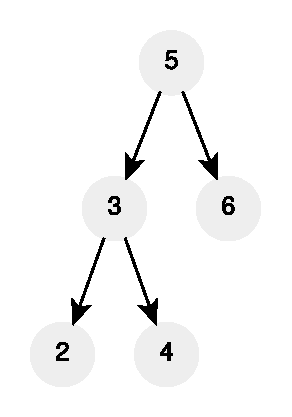
\includegraphics[width=\textwidth]{sources/max_gap/images/example1}
%	\caption[Sample short cpation]{Sample Caption}.
%	\label{fig:max_gap:example1}
%\end{figure}

\chapter{Fid the largest gap}
\label{ch:max_gap}
\section*{Introduction}

\section{Problem statement}
\begin{exercise}
\label{example:max_gap:exercice1}
Write a function that given a unsorted array $I$ of length $n$ returns the
largest gap between two elements appearing one next to the other (they are consecutive) 
when $I$ is sorted.
A gap between $x$ and $y$ is defined as the absolute value of the difference between $x$ and $y$: $|x-y|$.

	%example1
	\begin{example}
		\label{example:max_gap:example1}
		\hfill \\
		Given $I = \{5,3,1,8,9,2,4\}$ the function returns $3$. Sorting $I$ changes it into:
		$sort(I)= \{1,2,3,4,5,8,9\}$, and the largest gap between any two consecutive elements is $3$. In this case between $5$ and $8$.		
	\end{example}

	%example2
	\begin{example}
		\label{example:max_gap:example2}
		\hfill \\
		Given $I = \{7, 1, 8, 9,15\}$ the function returns $6$.
		$sort(I)= \{1,7,8,9,15\}$, and the largest gap between any two of its consecutive elements is $6$ e.g. between $1$ and $7$ or between $15$ and $9$.	
	\end{example}
	
\end{exercise}

\section{Clarification Questions}

\begin{QandA}
	\item 
	\begin{answered}
		\textit{}
	\end{answered}
	
\end{QandA}

\section{Discussion}
\label{max_gap:sec:discussion}


\subsection{Trivial Solution}
\label{max_gap:sec:trivial}

\begin{minipage}{\linewidth}
	\lstinputlisting[language=c++, caption={Sample Caption},label=list:max_gap]{sources/max_gap/max_gap_solution1.cpp}
\end{minipage}


\section{Radix Sort}
\label{max_gap:sec:radix_sort}

\section{Buckets and the pigeons holes}
\label{max_gap:sec:buckets}